%第4章:実験結果・考察
本章ではV字モデル開発に従って実装を行った。ここでは具体的な実装方法について述べる。
\section{実装・実験環境}
 実装に至っては2人のグループで行いエッジ処理側は真鍋樹が行った。ここではサーバ側の実装について述べる。ここではエッジ処理側のことをクライアントと呼ぶ。実装に使用したプログラム言語はクライアント、サーバどちらもPython3を使用した。


\subsection*{実験環境}
実験環境で使用したものを以下の表\ref{spec}に示す。
\begin{table}[htb]
\begin{center}
\caption{実行環境}
\begin{tabular}{|c|c|c|c|c|} \hline
処理担当 & OS & CPU & RAM & GPU \\ \hline
サーバ側 & Windows10 64bit Pro & Core2Duo E7500 2.93GHz & 4GB & GT740 \\ \hline
エッジ側 & RaspberryPi3B(Rasbian) & Broadcom 1.2GHz & 1GB & None \\ \hline
\end{tabular}
\label{spec}
	\end{center}
\end{table}


 実験環境で使用したライブラリ、プログラム言語を以下の表\ref{library_spec}に示す。
\begin{table}[htb]
\begin{center}
\caption{使用ライブラリ・使用言語}
\begin{tabular}{|c|c|c|c|c|} \hline
処理担当 & ライブラリ・使用言語名 & バージョン & 使用目的 \\ \hline \hline
サーバ側 & Python3 & 3.7.4 & メイン処理	\\ \hline
サーバ側 & OpenCV & 4.1.2 & 画像切り取り\\ \hline
サーバ側 & Yolo & 3 & バーコード領域取得\\ \hline
サーバ側 & CUDA & 10.1 & 学習に使用\\ \hline
サーバ側 & pyzbar & 0.1.8 & バーコード番号取得\\ \hline
サーバ側 & mysqlclient & 1.4.6 & DB操作\\ \hline \hline
Webページ & XAMPP & 3.2.4 & Webページ、DBホスト\\ \hline
Webページ & apache2 & 2.4.41 & Webページホスト\\ \hline
Webページ & MariaDB & 10.4.10 & DB\\ \hline
Webページ & PHP & 7.3.12 & Webページ処理、DB操作\\ \hline \hline
エッジ側 & Python3 & 3.7.3 & メイン処理		\\ \hline
エッジ側 & OpenCV & 3.4.3 & Webカメラ操作\\ \hline
\end{tabular}
\label{library_spec}
	\end{center}
\end{table}


\newpage

\subsection*{サーバ通信}
クライアントとのデータのやり取りを含めた連携には通信処理が必要不可欠になる。クライアントはセンサが反応したらカメラを起動し複数の画像を撮影する。つまりサーバに送られる画像データは1回につき1枚ではない。つまりクライアントが画像データを送信するデータサイズが不明のため、サーバ側では送信されたデータのどこからどの部分が1つの商品画像データになるのか判断できない。そこで、クライアントは画像データを送信する前に画像データの合計サイズを送信する。サーバは合計サイズ分だけデータを受信すれば続けて2回目のデータ送信が来ても1回目のデータと区別することができる。
クライアントから送られてきた画像データはバイナリ形式になっているのでOpenCV\cite{opencv}.のフォーマットに変換しなおしている。

\subsection*{Yoloによるバーコード領域特定}
Yoloを使用した理由は後述するpyzbar\cite{pyzbar}.の識別精度にある問題があったためである。pyzbar\cite{pyzbar}.は近距離で撮影したバーコードの画像の認識はうまくいくが、距離が離れると識別しなくなる。これは画像の中に占めるバーコード部分が少なくなってしまい認識がうまくいかないためと思われる。そこでYoloを使用し、画像からバーコードの部分のみの座標を取得する。バーコードの部分のみをpyzbarに渡すことで距離が離れていても近距離で撮影したのと同じ効果が得られるようになった。学習にはバーコードの画像を約2000枚用意した。Yoloの実行はサーバ側で行う。当初クライアント側であるRaspberryPiでYoloを実行すればサーバは不要になり通信におけるタイムラグもなくなることが期待されたが、残念ながらラズパイの性能ではYoloを高い識別精度を保ったままリアルタイムに動作させることは性能上難しかったためサーバで行うことになった。

\subsection*{DBを使用した商品情報の管理}
カゴの中の商品を管理と、商品自体の情報の管理にDBを使用した。商品MariaDBを使用した。カゴDBの構造を以下に示す。
初めに商品自体のデータを管理するitemテーブルを表\ref{item_db}に示す。janはJANコードのことであり、商品識別番号のことである。titleは商品名のことである。price商品の価格を示す。
image\_urlは商品の画像があるURLを示している。最後のimage\_rawはこのシステムでは使用していないが、画像データそのものを格納できるようにしている。
\begin{table}[htbp]
\centering
\caption{itemテーブル}
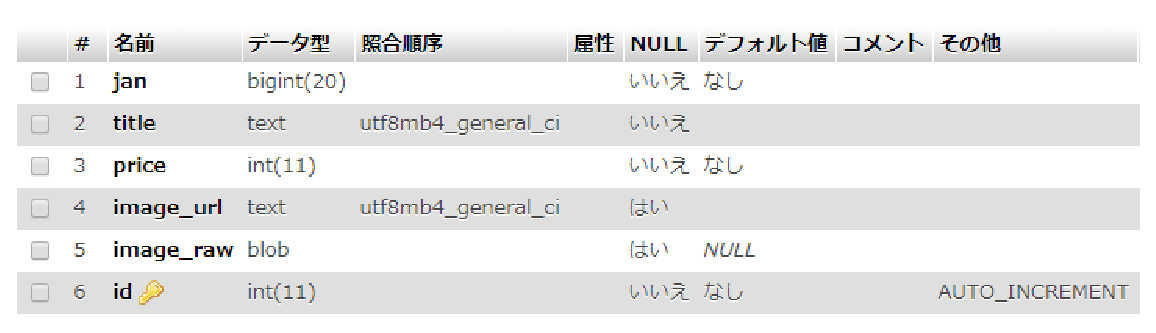
\includegraphics[width=15cm]{./pic/item_db.eps}
\label{item_db}
\end{table}

\newpage

次にカートのテーブルcartテーブルの構造を表\ref{cart_db}に示す。id行の固有番号を示すためにある。この番号をでカートごとの区別を行う。janはJANコードのことである。cart\_idはカートの固有番号を示す。この番号があることで複数運用した際も区別することができる。
%%%商品DB
\begin{table}[htbp]
\centering
\caption{cartテーブル}
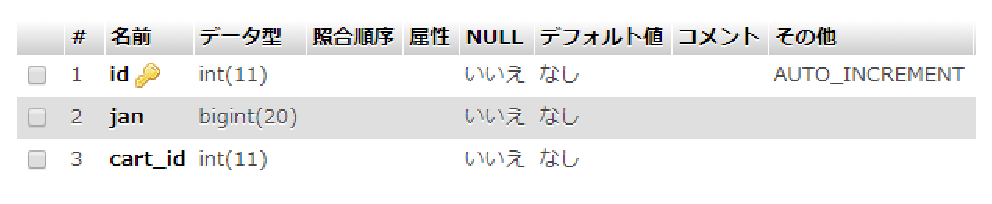
\includegraphics[width=15cm]{./pic/cart_db.eps}
\label{cart_db}
\end{table}


顧客テーブルの構造を表\ref{customer_db}に示す。この顧客テーブルはシステムの動作テストを行う際に必要だったため作成した。動作用に仮の顧客情報を管理する。idは顧客の固有番号を示し、balanceは顧客の所持金額を示す。

\begin{table}[htbp]
\centering
\caption{customerテーブル}
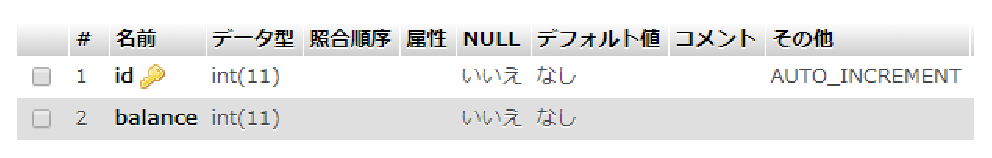
\includegraphics[width=15cm]{./pic/customer.eps}
\label{customer_db}
\end{table}

\newpage

\subsection*{決済システム}
設計では決済システムが動作するのはユーザが退店する際に自動で行われることになっているがその機能を実装するには時間の都合上難しいと判断したため、仮の決済用Webページを作成して代用している。ページ作成にはPHPを使用している。以下にWebページでの動作の流れを示す。

\subsection*{カート画面}
本来はユーザがこのような画面を操作することなく自動で決済が行われるのでこれは動作テスト用に作成している。以下の図\ref{web_cart}は初めにどのカートを使用しているかを選択するためにある。
\begin{figure}[htbp]
\centering
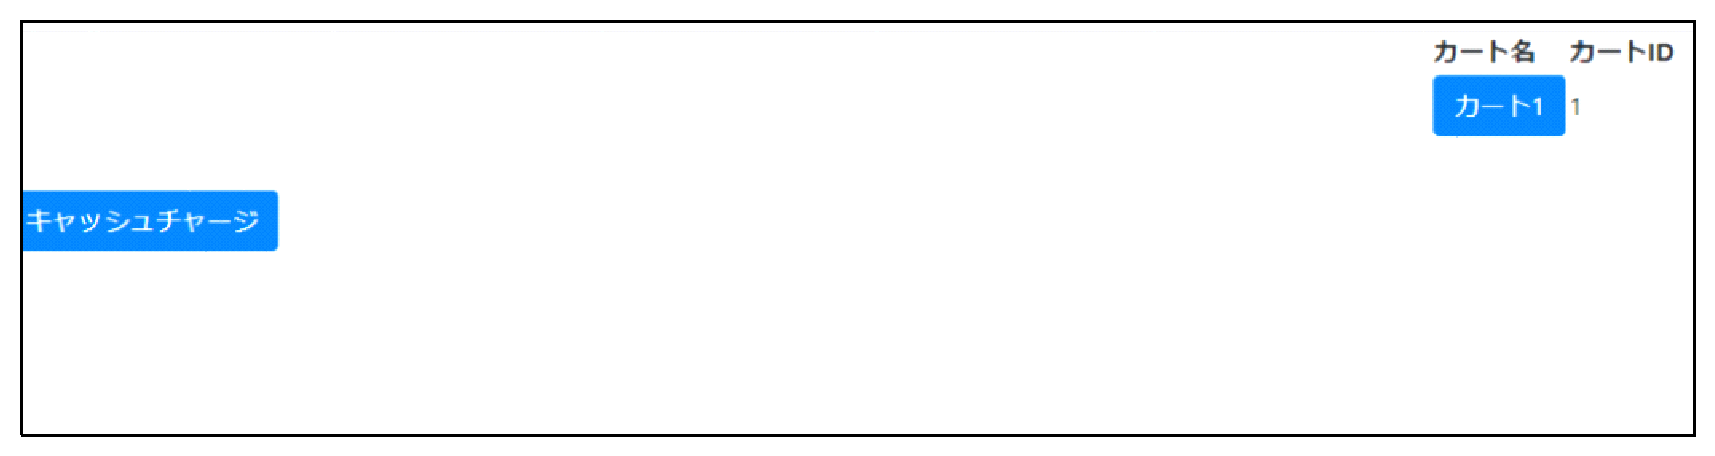
\includegraphics[width=15cm]{./pic/web/1.eps}
\caption{Webページ カート画面}
\label{web_cart}
\end{figure}

\subsection*{カート内商品一覧}
こちらの図\ref{web_cart_items}はカート内にある購入予定の商品の一覧を表している。表示内容は商品名と価格、商品画像と個数の4つである。ページ内にある緑のボタンを押すと会計が行われる。
\begin{figure}[htbp]
\centering
\includegraphics[width=15cm]{./pic/web/2.eps}
\caption{Webページ カート内商品一覧}
\label{web_cart_items}
\end{figure}

\subsection*{決済完了画面}
図\ref{web_cart_items}のページでボタンを押すと図\ref{web_checksum}画面に移行し、顧客の所持金から購入金額が差し引かれ、残高が表示される。また、所持金が購入金額が下回っていた場合は所持金額が足りないと警告され会計は行われない。
\begin{figure}[htbp]
\centering
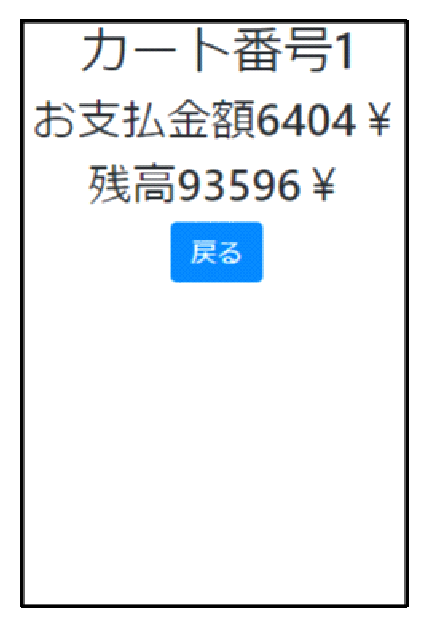
\includegraphics[width=10cm,height=10cm]{./pic/web/3.eps}
\caption{Webページ 決済完了}
\label{web_checksum}
\end{figure}

\newpage

\section{検証}
V字モデルに従って4.1節で述べた実装部分に関するテストを行うことで要件を満たしているかどうかを確認する。以下にそれぞれのテスト項目を表で示す。

\subsection*{サーバ通信}
サーバ通信の検証で行った単体テストを以下の表\ref{server_test}に示す。
\begin{table}[htbp]
\centering
\caption{サーバ通信単体テスト}
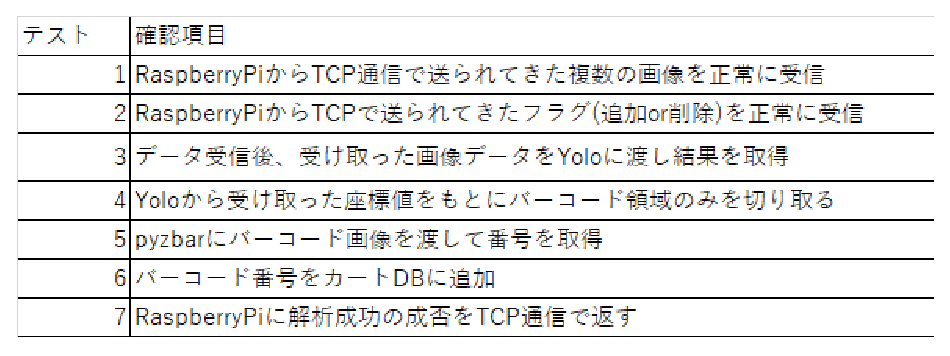
\includegraphics[width=12cm]{./pic/server_test.eps}
\label{server_test}
\end{table}

\subsection*{Yoloによるバーコード領域特定}
Yoloにおけるバーコード検知の検証で行った単体テスト項目を以下の表\ref{yolo_test}に示す。
\begin{table}[htbp]
\centering
\caption{Yoloによるバーコード領域特定単体テスト}
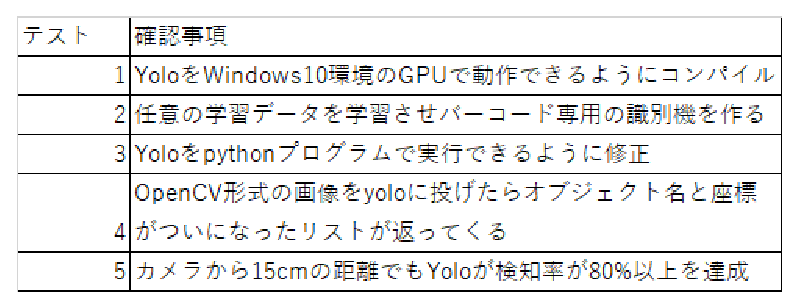
\includegraphics[width=12cm]{./pic/yolo_test.eps}
\label{yolo_test}
\end{table}

\subsection*{DBを使用した商品情報の管理}
DBを使用した商品情報の管理の単体テストを以下の表\ref{table_test}に示す。

\begin{table}[htbp]
\centering
\caption{DBテーブル単体テスト}
\includegraphics[width=12cm]{./pic/table_test.eps}
\label{table_test}
\end{table}


\subsection*{決済システム}
決済システムにおける単体テストを以下の表\ref{db_test}に示す
\begin{table}[htbp]
\centering
\caption{決済システム単体テスト}
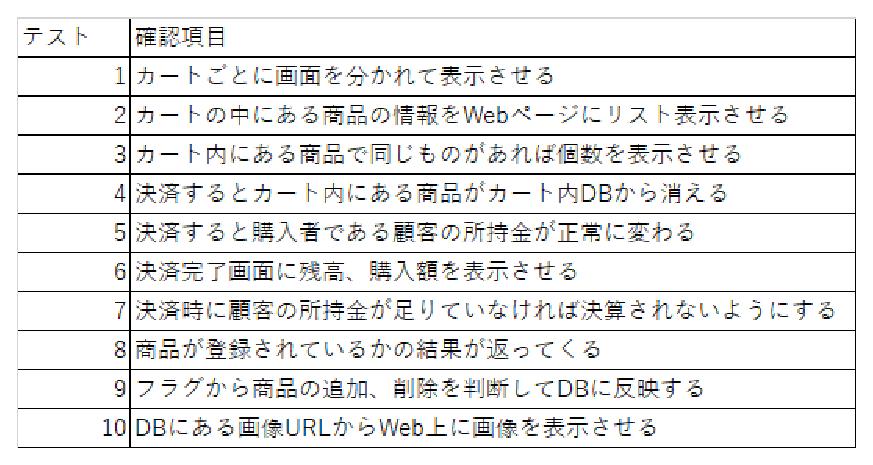
\includegraphics[width=12cm]{./pic/db_test.eps}
\label{db_test}
\end{table}

\newpage

これらの単体テスト項目を満たしていることを確認することにより、システムが表\ref{join_test}の結合テストの項目を満たしていることを確認する。結合テストではシステムの中で筆者が実装担当したサーバ部分の項目が記されている。

\begin{table}[htbp]
\centering
\caption{結合テスト}
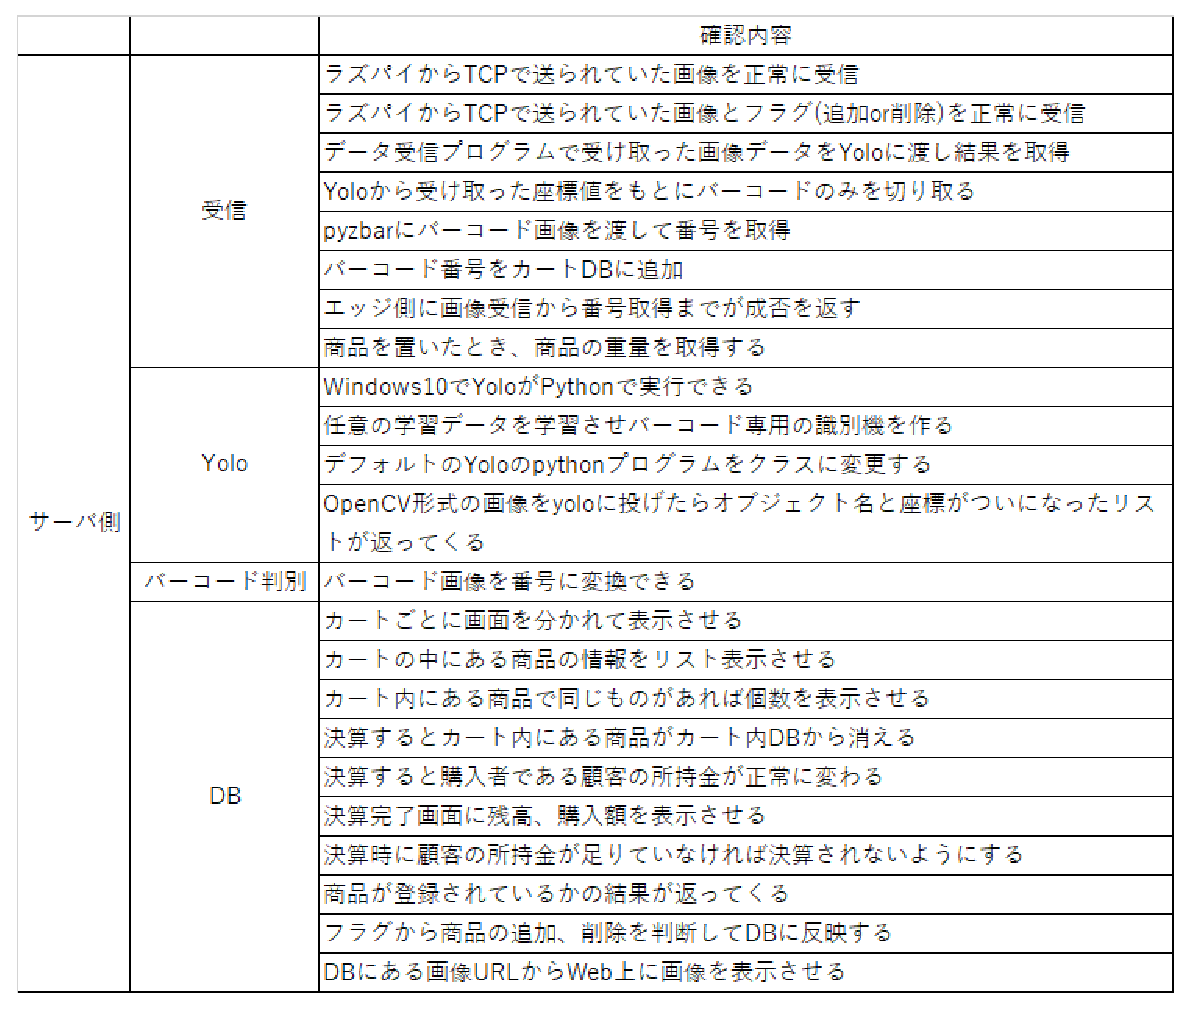
\includegraphics[height=15cm,width=15cm]{./pic/join_test.eps}
\label{join_test}
\end{table}

\newpage

結合テストの内容を確認し、各モジュール間でのデータの受け渡しが正常に行われていることを確認する。最後に表\ref{integrated_test}に総合テストの内容を示す。総合テストではユーザが買い物をはじめ最後に決済するまでの流れをシナリオとしている。このシナリオではユーザの残高は購入予定金額を下回らないと想定し、また買い物キャンセルすることはないという想定になっている。

\begin{table}[htbp]
\centering
\caption{総合テスト}
\includegraphics[width=15cm]{./pic/integrated_test.eps}
\label{integrated_test}
\end{table}

 
